%This file will discuss project results (validation of solution)
%This file should be included in doc using \input{file}

\section{Project Results}

\subsection{Simulations}
\subsection{Hover Test}
Using the models and systems discussed in the previous subsection, our preliminary flight simulation was constructed.  The SimuLink model Dynamic\_Simulation.slx was created.  The altitude controller was tested by providing a step input.  After some tuning of the controller, we were able to obtain the following step response.

\begin{figure}[h]
	\centering
	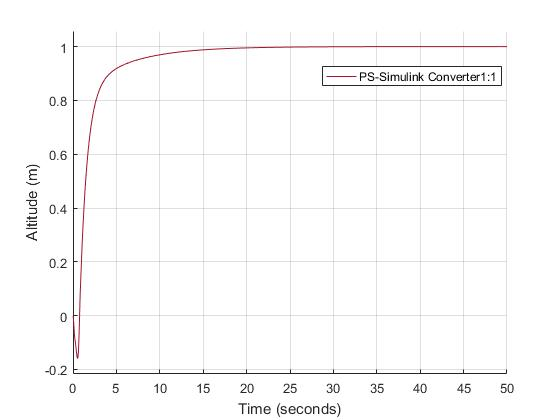
\includegraphics[scale = 0.5]{stepresponse.jpg}
	\caption{Hovering Step Response, for 1 metre altitude.}
	\label{fig:1m_step}
\end{figure}

When this test was initially performed, the SimScape MultiBody physical simulation did not yet include a model for a hard stop at the origin of the Z axis.  This is to say that there was no representation of ground for the quad-rotor drone to rest upon.  This is why an initial decline in position can be seen in the graph.  This was subsequently added this term.

Further tests to be performed during the week will outlined in Section \ref{discussion:sim}.



\subsection{Physical Implementation}


\subsection{Graphical User Interface}

